% ----------------------------------------------------
% Subsystem Design
% ----------------------------------------------------
\documentclass[class=report,11pt,crop=false]{standalone}
% Page geometry
\usepackage[a4paper,margin=20mm,top=25mm,bottom=25mm]{geometry}

\newcommand{\tabitem}{~~\llap{\textbullet}~~}
% Font choice
\usepackage{lmodern}

\usepackage{lipsum}

% Use IEEE bibliography style
\bibliographystyle{IEEEtran}

% Line spacing
\usepackage{setspace}
\setstretch{1.20}

% Ensure UTF8 encoding
\usepackage[utf8]{inputenc}

% Language standard (not too important)
\usepackage[english]{babel}

% Skip a line in between paragraphs
\usepackage{parskip}

% For the creation of dummy text
\usepackage{blindtext}

% Math
\usepackage{amsmath}

% Header & Footer stuff
\usepackage{fancyhdr}
\pagestyle{fancy}
\fancyhead{}
\fancyhead[R]{\nouppercase{\rightmark}}
\fancyfoot{}
\fancyfoot[C]{\thepage}
\renewcommand{\headrulewidth}{0.0pt}
\renewcommand{\footrulewidth}{0.0pt}
\setlength{\headheight}{13.6pt}

% Epigraphs
\usepackage{epigraph}
\setlength\epigraphrule{0pt}
\setlength{\epigraphwidth}{0.65\textwidth}

% Colour
\usepackage{color}
\usepackage[usenames,dvipsnames]{xcolor}

% Hyperlinks & References
\usepackage{hyperref}
\definecolor{linkColour}{RGB}{77,71,179}
\hypersetup{
    colorlinks=true,
    linkcolor=linkColour,
    filecolor=linkColour,
    urlcolor=linkColour,
    citecolor=linkColour,
}
\urlstyle{same}

% Automatically correct front-side quotes
\usepackage[autostyle=false, style=ukenglish]{csquotes}
\MakeOuterQuote{"}

% Graphics
\usepackage{graphicx}
\graphicspath{{Images/}{../Images/}}
\usepackage{makecell}
\usepackage{transparent}

% SI units
\usepackage{siunitx}

% Microtype goodness
\usepackage{microtype}

% Listings
\usepackage[T1]{fontenc}
\usepackage{listings}
\usepackage[scaled=0.8]{DejaVuSansMono}

% Custom colours for listings
\definecolor{backgroundColour}{RGB}{250,250,250}
\definecolor{commentColour}{RGB}{73, 175, 102}
\definecolor{identifierColour}{RGB}{196, 19, 66}
\definecolor{stringColour}{RGB}{252, 156, 30}
\definecolor{keywordColour}{RGB}{50, 38, 224}
\definecolor{lineNumbersColour}{RGB}{127,127,127}
\lstset{
  language=Matlab,
  captionpos=b,
  aboveskip=15pt,belowskip=10pt,
  backgroundcolor=\color{backgroundColour},
  basicstyle=\ttfamily,%\footnotesize,        % the size of the fonts that are used for the code
  breakatwhitespace=false,         % sets if automatic breaks should only happen at whitespace
  breaklines=true,                 % sets automatic line breaking
  postbreak=\mbox{\textcolor{red}{$\hookrightarrow$}\space},
  commentstyle=\color{commentColour},    % comment style
  identifierstyle=\color{identifierColour},
  stringstyle=\color{stringColour},
   keywordstyle=\color{keywordColour},       % keyword style
  %escapeinside={\%*}{*)},          % if you want to add LaTeX within your code
  extendedchars=true,              % lets you use non-ASCII characters; for 8-bits encodings only, does not work with UTF-8
  frame=single,	                   % adds a frame around the code
  keepspaces=true,                 % keeps spaces in text, useful for keeping indentation of code (possibly needs columns=flexible)
  morekeywords={*,...},            % if you want to add more keywords to the set
  numbers=left,                    % where to put the line-numbers; possible values are (none, left, right)
  numbersep=5pt,                   % how far the line-numbers are from the code
  numberstyle=\tiny\color{lineNumbersColour}, % the style that is used for the line-numbers
  rulecolor=\color{black},         % if not set, the frame-color may be changed on line-breaks within not-black text (e.g. comments (green here))
  showspaces=false,                % show spaces everywhere adding particular underscores; it overrides 'showstringspaces'
  showstringspaces=false,          % underline spaces within strings only
  showtabs=false,                  % show tabs within strings adding particular underscores
  stepnumber=1,                    % the step between two line-numbers. If it's 1, each line will be numbered
  tabsize=2,	                   % sets default tabsize to 2 spaces
  %title=\lstname                   % show the filename of files included with \lstinputlisting; also try caption instead of title
}

% Caption stuff
\usepackage[hypcap=true, justification=centering]{caption}
\usepackage{subcaption}

% Glossary package
% \usepackage[acronym]{glossaries}
\usepackage{glossaries-extra}
\setabbreviationstyle[acronym]{long-short}

% For Proofs & Theorems
\usepackage{amsthm}

% Maths symbols
\usepackage{amssymb}
\usepackage{mathrsfs}
\usepackage{mathtools}

% For algorithms
\usepackage[]{algorithm2e}

% Spacing stuff
\setlength{\abovecaptionskip}{5pt plus 3pt minus 2pt}
\setlength{\belowcaptionskip}{5pt plus 3pt minus 2pt}
\setlength{\textfloatsep}{10pt plus 3pt minus 2pt}
\setlength{\intextsep}{15pt plus 3pt minus 2pt}

% For aligning footnotes at bottom of page, instead of hugging text
\usepackage[bottom]{footmisc}

% Add LoF, Bib, etc. to ToC
\usepackage[nottoc]{tocbibind}

% SI
\usepackage{siunitx}

% For removing some whitespace in Chapter headings etc
\usepackage{etoolbox}
\makeatletter
\patchcmd{\@makechapterhead}{\vspace*{50\p@}}{\vspace*{-10pt}}{}{}%
\patchcmd{\@makeschapterhead}{\vspace*{50\p@}}{\vspace*{-10pt}}{}{}%
\makeatother
\begin{document}
% ----------------------------------------------------
\chapter{Subsystem Design} \label{ch:design}
\vspace{-1cm}
% =====================================================
\section{Design Decisions}


\subsection{Final Design}
% 2. Provide the final schematic, make sure to include:
%       - labels and component values
%       - descriptions/comments on different parts of the schematic
%       - the completed schematic page setup: title, date, revision number, author name and surname.
%       - power flags on all power connections (3V, 5V, Gnd, etc)
% 2. Provide the final PCB, make sure to include:
%       - front, back and 3D view 
\begin{figure}[htbp]
    \centering
    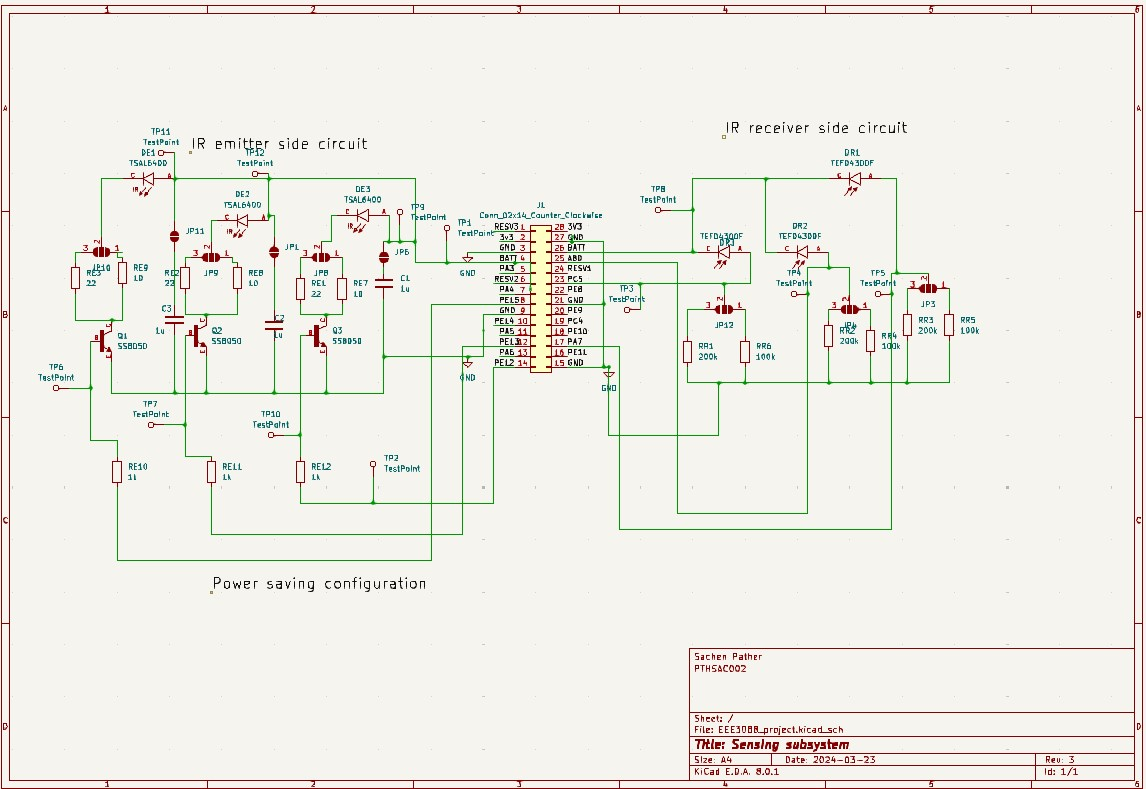
\includegraphics[width=1.1\linewidth]{EEE3088F_final_report_latex_template-2//Figures/Final_Schematic_4.jpg}
    \caption{Final Schematic}
    \label{fig:schematic}
\end{figure}

\begin{figure}[htbp]
    % First subfigure
    \begin{subfigure}[b]{0.6\linewidth}
        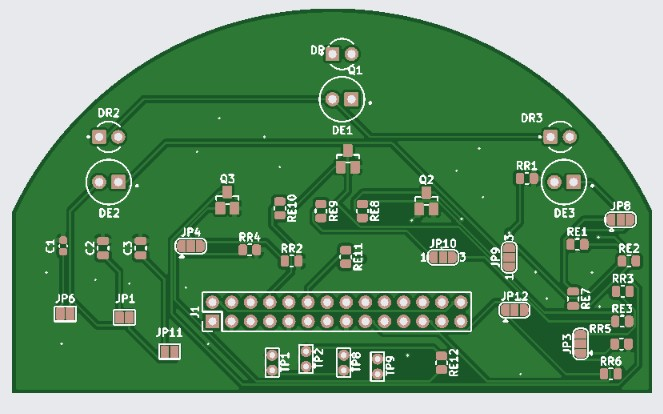
\includegraphics[width=\linewidth]{EEE3088F_final_report_latex_template-2//Figures/Front_PCB.jpg}
        \caption{Front PCB}
        \label{fig:PCB_Front}
    \end{subfigure}
    \hrule % Horizontal line
    % Second subfigure
    \begin{subfigure}[b]{0.6\linewidth}
        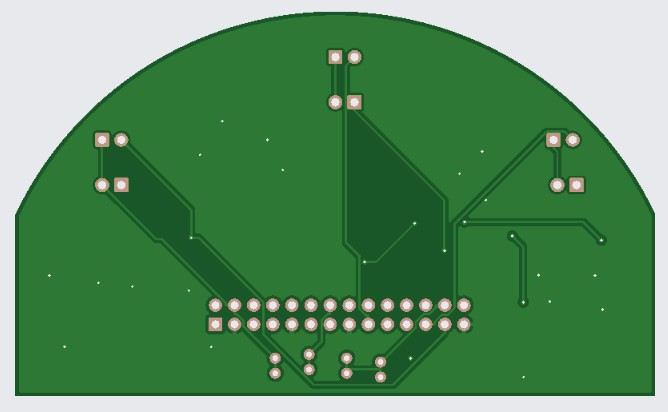
\includegraphics[width=\linewidth]{EEE3088F_final_report_latex_template-2//Figures/Back_PCB.jpg}
        \caption{Back PCB}
        \label{fig:PCB_back}
    \end{subfigure}
    \hrule % Horizontal line
    % Third subfigure
    \begin{subfigure}[b]{0.6\linewidth}
        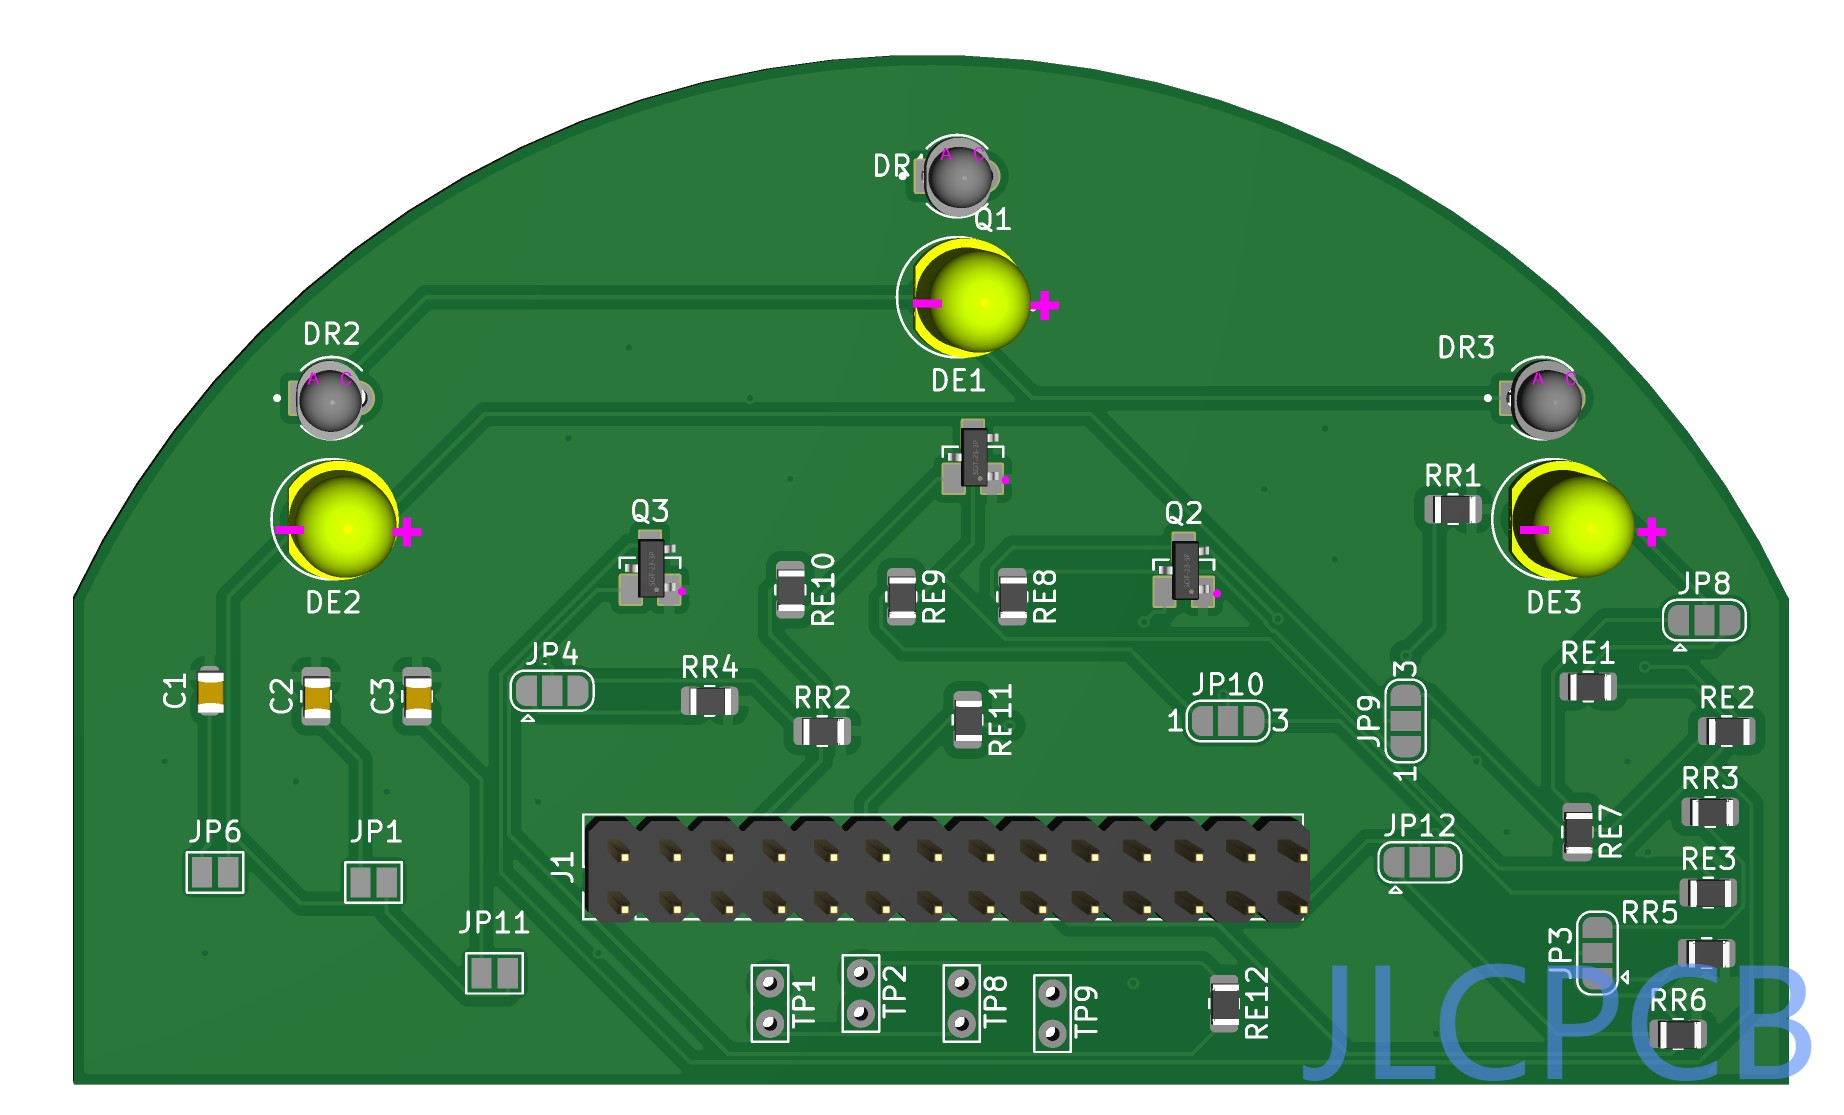
\includegraphics[width=\linewidth]{EEE3088F_final_report_latex_template-2//Figures/3D_Model_2.jpg}
        \caption{3D PCB}
        \label{fig:PCB_3D}
    \end{subfigure}
    \caption{PCB}
    \label{fig:PCB}
\end{figure}
\\
The first design decision to take into consideration was the selection of the infrared LED emitters and infrared sensors as these will be responsible for the main application of the subsystem - the detection of walls and obstacles. The following tables below describe the design decisions with regards to choosing these components:

\begin{table}[h]
  \begin{center}
    \caption{Tabulation of design decision for IR Emitter}
    \label{tab:IR emitters}
    \begin{tabular}{|>{\centering\arraybackslash}m{2cm}|m{3.5cm}|m{5cm}|m{6.5cm}|}
      \hline
      \textbf{Component} & \textbf{Description} & \textbf{Advantages} & \textbf{Disadvantages}\\   
      \hline
      TSAL6400 & 
      \begin{itemize}
      \item 25mW/sr @ 100mA 
      \item Vf = 1.35V 
      \item Peak Wavelength = 940 nm 
      \item Plugin, D=5mm 
      \end{itemize} &
      \begin{itemize}
      \item High radiant intensity for good transmission range 
      \item Compact 5mm package size is convenient for PCB mounting 
      \item High number in stock 
      \end{itemize} &
      None significant for this application \\
      \hline
      TSAL4400 & 
      \begin{itemize}
      \item 16mW/sr @ 100mA 
      \item Vf = 1.35V 
      \item Peak Wavelength = 940 nm 
      \item Plugin, D=2.9mm 
      \end{itemize} &
      \begin{itemize}
      \item Slightly smaller package size can be beneficial for tight spaces 
      \item High number in stock 
      \end{itemize} &
      Lower radiant intensity may result in reduced transmission range \\
      \hline 
      SFH 4550 & 
      \begin{itemize}
      \item 1100mW/sr @ 100mA 
      \item Vf = 1.5V 
      \item Peak Wavelength = 860 nm 
      \item Plugin, D=5.7mm  
      \end{itemize} &
      \begin{itemize}
      \item Extremely high radiant intensity for maximum transmission range  
      \end{itemize} &
      \begin{itemize}
      \item Larger package size may not be ideal for compact designs 
      \item Higher radiant means higher power dissipation and thermal management need 
      \item Low number in stock
      \end{itemize} \\
      \hline
    \end{tabular}
  \end{center}
\end{table} \\ 
 Considering the above components, the decision on which component to use is the TSAL6400. Its radiant intensity of 25mW/sr @ 100mA strikes a good balance between sufficient transmission range and power dissipation/thermal management needs. Meanwhile the TSAL4400 is a lighter weight, lower intense version of the TSAL6400. The SFH 4550 has extremely high intensity which would be ideal, however considering the power dissipation in the circuit, it is not best suited for the micro-mouse application as it would greatly reduce battery life. The slightly larger size is also less ideal.
\\\\ %Series Resistor selection
In conjuction with the TSAL6400, a resistor value can be calculate which enables the maximum radiant intensity. Using the datasheet values from the TSAL6400: Maximum Rated Forward Current (IF): 100 mA
Radiant Intensity (Ie) at IF = 100 mA: 25 mW/sr typical, up to 125 mW/sr max.\\
The needed series resistor value can be calculated using:\\
R = (Vsupply - VF) / IF\\
Assuming the maximum 1.6V forward voltage at 100 mA:\\
R = (3.7V - 1.6V) / 0.1A = 21 ohms
\\
So driving the LED at its maximum rated 100 mA forward current will provide the highest radiant intensity output. So a 22ohm resistor is to be selected, using a surface mount SMD-0805 resistor series. A 10ohm resistor is provided as another option on the schematic with a solder jumper in the case the input voltage is lower than 3.7V and more current needs to be drawn however this will likely not be used.
\\\\
A bypass capacitor will also be used to filter out unwanted frequencies such as noise. You would generally want to pass frequencies up to several hundred kHz without significant attenuation in IR circuits.
Assume you want to pass frequencies up to 1MHz (-3dB bandwidth):
Desired max impedance = 10\% of LED's dynamic resistance \\
= 0.1 * (1.6V / 100mA) = 0.16Ω \\
At 1MHz, Xcap = 1/(2pifC) \\
0.16 = 1/(2pi1MHzC) \\
C = 1uF

So a 1uF bypass capacitor would be a good choice to minimize impedance up to 1MHz. A surface mount ceramic capacitor smd: C\_0805 series capacitor of value 1uF is therefore chosen. A lower capacitor value will lead to a higher impedance which limits the bypass effectiveness.

\\
\begin{table}[h]
  \begin{center}
    \caption{Tabulation of design decision for IR Receiver}
    \label{tab:IR emitters}
    \begin{tabular}{|>{\centering\arraybackslash}m{2cm}|m{3.5cm}|m{5cm}|m{6.5cm}|}
      \hline
      \textbf{Component} & \textbf{Description} & \textbf{Advantages} & \textbf{Disadvantages}\\   
      \hline
      TEFD4300F & 
      \begin{itemize}
      \item 60V 950nm 770nm~1070nm ±20° 150pA Plugin,D=3mm Photodiodes
      
      \end{itemize} &
      \begin{itemize}
      \item Low 0.15nA typical dark current 
      \item 3mm compact package size
      \item Specified ±20° angle of half-sensitivity, matched to emitter 
      
      \end{itemize} &
      \begin{itemize}
      \item Slightly narrower 770nm - 1070nm spectral bandwidth
      \end{itemize}
      \\
      \hline
      SFH203PFA  & 
      \begin{itemize}
      \item 50V 900nm 750nm~1100nm 1nA Plugin,D=4.8mm Photodiodes
      \end{itemize} &
      \begin{itemize}
            \item Higher Wide 750nm - 1100nm spectral bandwidth 
      \item Fast 5ns rise/fall times
     
      \end{itemize} &  
      \begin{itemize}
     \item Higher 1nA typical dark current 
      \item No specific angle of half-sensitivity provided on datasheet 
      \end{itemize}
      \\
      \hline  
      XYC-PD333B-L2 & 
      \begin{itemize}
      \item 35V 940nm 760nm~1100nm 10nA Plugin,D=5mm Photodiodes 
 
      \end{itemize} &
      \begin{itemize}
      \item Wide ±30° angle of half-sensitivity 
      \item 5mm through-hole package, easy mounting

      \end{itemize} &
    \begin{itemize}
      \item Higher 10nA typical dark current
      \item Limited datasheet details on some parameters
      \end{itemize}
      \\
      \hline
    \end{tabular}
  \end{center}
\end{table}


  The TEFD4300F is selected as the best choice because the ±20° angle matches well with the ±20° emission angle of the TSAL6400 IR LED transmitter, The 770nm - 1070nm bandwidth aligns nicely with the 940nm peak wavelength of the IR LED, Extremely low 0.15nA typical dark current for high signal-to-noise ratio and it has a comprehensive datasheet gives confidence in designed-in parameters.\\
  With regards to the options available, availability and cost is no issue as all 3 are well within the allocated budget. The TEFD4300F provides the best balance of optical characteristics, voltage ratings, dark current, and available specifications - making it well-suited for reliable operation with the 3.7V bias in this IR receiver application. \\\\
  To properly bias the TEFD4300F photodiode with the 3.7V supply for measuring the output voltage, a relatively high value resistor in series needs to be used. This will provide a reverse bias voltage across the photodiode while limiting the current draw. Given the values from the datasheet: Maximum reverse voltage rating (VR) = 60V,
Typical reverse dark current (Iro) at VR = 10V is 0.15nA,
Maximum reverse light current (Ira) at 1mW/cm2, 950nm, and VR = 5V is 27μA\\
R = V / I \\
= 3.7V / 27μA\\
= 137kΩ as a minimum\\
Therefore a selection of a 200kΩ is selected. A solder jumper that has a 100kΩ resistor is also provided as an option in the case the voltage input from the battery is much lower than expected.
\\
An output voltage is then taken and fed into an analogue input, this analogue input will be used and an ADC will be used to convert the analogue signal to a digital signal to light up the LED and so that the system reacts accordingly..
\\\\
This is now responsible for the majority of the functionality of the circuit. The next design decision is deciding how to incorporate a power saving mode. The power saving mode section of the circuit makes use of a transistor configuration which is used as a switch, with the collector of each transistor connected to to series IR Emitter and resistor combination, the base connected to the PWM output pin, and the emitter to ground. The PWM output pin on the microcontroller is responsible for changing the duty cycle i.e When the PWM signal is LOW, no base current flows into the NPN transistor, so the transistor is in cut-off mode and not conducting. This means no current flows through the LED, and it is off. Similarly when PWM is high, the IR LED illuminates at its maximum rated current set by the current limiting resistor. Hence it  can be seen changing the pwm duty cycle affects the average current per unit time hence can be used to save power at duty cycle = 50\%.\\\\
Another design decision had to be made with regards to using the pwm output in seres with the IR Emitter and resister combination in place of the battery and using it to drive the base of the transistor which can be used as a switch. \\
\begin{table}[h]
  \centering
    \caption{Tabulation of design decision for Power saving configuration}
    \label{tab:Power saving configurations}
    \begin{tabular}{|>{\centering\arraybackslash}m{3cm}|m{5cm}|m{7cm}|}
      \hline
      \textbf{Configuration} & \textbf{Advantages} & \textbf{Disadvantages}\\   
      \hline
      PWM driving the transistor base as a switch: & 
      \begin{itemize}
      \item Simple drive circuitry, just a base resistor 
      \item LED either fully on or fully off
      \item Maximum available supply voltage across LED when on
      \item 2 distinct modes i.e a power saving mode and a fully on mode 
      \end{itemize} &
      \begin{itemize}
      \item Generates sharp LED current transitions that may produce Electromagnetic interference  
      \item LED always operates at maximum current
      \end{itemize}\\
      \hline
      PWM powering the IR Led: & 
      \begin{itemize}
      \item Simple Flexibility to adjust LED brightness continuously 
      \item Allows analog modulation of LED current/intensity below maximum
      \item Can improve efficiency at lower brightness levels by reducing LED power
      \item Smoother LED current transitions may reduce EMI 
      \end{itemize} &
      \begin{itemize}
      \item Supply voltage limitations may prevent using full LED power at maximum brightness 
      \item Does not distinctly give 2 different modes but this could be hard coded
      \end{itemize}\\
      \hline
    \end{tabular}
\end{table}
\\
Using the pwm to drive the base of the transistor was then selected. This is mainly due to simplicity with regards to coding the pwm of having one distinct power saving mode and one fully on mode, and also now knowing the supply voltage limitations of the pwm to power the IR Led. Hence the average current per unit time will change based on the duty cycle.\\
For the IR receiver side circuit, another design decision was to be considered but this will not be discussed in depth. The output voltage from the series receiver resistor configuration is fed into an analogue input. Instead of directly feeding into the analogue input, we have had to consider using an amplifier transistor configuration to give a distinct high and low at a certain output voltage which would then be fed into the analogue input. The issue with this is right now I am unsure which output voltage would be necessary for the transistor to turn on in practical use and this would affect the value at the base of the transistor so unwanted issues with the circuit may occur. \\\\
\textbf{Final solution description} \\
IR Emitter circuit:\\
TSAL6400 IR LED was chosen for its balance of high radiant intensity (25mW/sr @ 100mA) and compact 5mm package size. To drive the LED at its maximum 100mA rated current, a 22Ω series resistor was calculated. Additionally, a 1μF bypass capacitor was added to filter out noise up to 1MHz frequencies.
\\IR Receiver circuit:\\
For the IR receiver, the TEFD4300F photodiode was selected due to its matched ±20° angle, 770-1070nm bandwidth, extremely low 0.15nA dark current, and comprehensive datasheet. A 200kΩ series resistor was utilized to provide proper 3.7V reverse bias while ensuring current remains within the photodiode ratings. The output voltage from the photodiode/resistor is fed into a microcontroller analog input.
\\Power Saving Mode circuitry:\\
The implementation of the power saving mode involved using an NPN transistor with its base driven by a PWM signal from the microcontroller. When the PWM signal is high, the transistor conducts, allowing maximum rated current through the IR LED. Conversely, when the PWM signal is low, the transistor cuts off the LED current for power saving. Varying the PWM duty cycle modulates the average LED power/brightness. This configuration was favored over directly driving the LED with PWM due to its simplicity in coding two distinct modes (full power vs power saving) and ensuring maximum LED output when needed.

  
% =====================================================
\section{Failure Management}

\begin{table}[h]
    \centering
    \caption{Failure Management Components} 
    \label{tab:failuremanagement}
    \begin{tabular}{|p{5cm}|p{10cm}|}
        \hline
        \textbf{Name} & \textbf{Description} \\
        \hline
        - IR Emitter circuit Battery & Use Test point TP1 to verify if the battery provides the required output voltage. \\
        \hline
        - Alternative Resistances, Solder Jumpers JP8, JP9, JP10 & If the battery outputs a lower voltage, solder jumpers can be connected to alternate resistors as per the schematic. \\
        \hline
        - Unwanted Capacitor Impedances, Jumpers JP6, JP1, JP11 & In case capacitors introduce unwanted impedance affecting the circuit, these jumpers can be disconnected. \\
        \hline
        - IR Receiver circuit Battery & Similar to IR Emitter battery, use Test point TP8, used to verify battery output voltage. \\
        \hline
        - Alternative Resistances, Solder Jumpers JP12, JP4, JP3 & Similar to IR Emitter, alternative resistors can be selected if battery voltage is low. \\
        \hline
        - Output Voltage Test & Verify the output voltages are correct using (TP3, TP4, TP5) when necessary i.e at a distance away from a wall. \\
        \hline
        - Alternative Resistances, Solder Jumpers JP12, JP4, JP3 & If the battery outputs a lower voltage, solder jumpers can be connected to alternate resistors as per the schematic. Also if output voltage needs to be adjusted, resistor can change. \\
        \hline
        - IR LED activity check & Use test points (TP11, TP12, TP9) and solder jumpers (JP10,JP9,JP8) to measure voltage drop between the 2 points. \\
        \hline
        - Transistor activity check & Use test points (TP6, TP7, TP10) to measure voltage across BE junction of NPN transistor (i.e voltage between test point and ground) when PWM duty cycle is 100\% and 0\%. \\
        \hline
        - IR photodiode activity check & Use test points (TP8) and solder jumpers (JP12,JP4,JP3) to measure voltage drop between the 2 points. \\
        \hline
    \end{tabular}
\end{table}

% =====================================================
\section{System integration and Interfacing}
    \centering
    \caption{System Interfacing table}
    \label{tab:my-table}
    \begin{tabular}{|c|c|c|c|p{7cm}|}
        \hline
        \textbf{Interface} & \textbf{Pin-S} & \textbf{Pin-M} & \textbf{Associated to} & \textbf{Use in Circuit} \\
        \hline
        I01 & 4 & Battery & BATT & Voltage source, connected to IR Emitter side circuits Voltage input, i.e +ve terminals of DE1, DE2, DE3 and +ve terminals of C1, C2, C3 \\
        \hline
        I02 & 8 & 24 & PE15 & PWM1: Used to drive base of transistor Q1 in Power Saving configuration through RE10 using pulse width modulation controlling the duty cycle \\
        \hline
        I03 & 9 & 23 & GND & Ground connection for Q1, Q2, Q3 emitters and C1, C2, C3 -ve terminals \\
        \hline
        I04 & 12 & 26 & PE13 & PWM2: Used to drive base of transistor Q2 in Power Saving configuration through RE11 using pulse width modulation controlling the duty cycle \\
        \hline
        I05 & 14 & 27 & PE12 & PWM3: Used to drive base of transistor Q3 in Power Saving configuration through RE12 using pulse width modulation controlling the duty cycle\\
        \hline
        I06 & 15 & 23 & GND & Ground connection for (RR1 or RR6), (RR2 or RR4), (RR3 or RR5) \\
        \hline
        I07 & 17 & 38 & PA7 & Analog12: Analog Input - Output Voltage from IR Receiver circuit, Wire connected to DR1\_Right +ve terminal and JP3 (RR3 or RR5) \\
        \hline
        I08 & 23 & 36 & PC5 & Analog14: Analog Input - Output Voltage from IR Receiver circuit, Wire connected to DR3\_Left +ve terminal and JP12 (RR1 or RR6) \\
        \hline
        I09 & 25 & ? & AB0 & Analog15: Analog Input - Output Voltage from IR Receiver circuit, Wire connected to DR2\_Middle +ve terminal and JP4 (RR2 or RR4) \\
        \hline
        I10 & 26 & Battery & BATT & Voltage Source, connected to IR Receiver side circuits Voltage input, i.e -ve terminals of DR1, DR2, DR3 \\
        \hline
    \end{tabular}
\end{table}


- Pin-S is the Sensor Subsystem pin headers,makes use of 2x14 (2.54mm pin pitch) connector \\
- Pin-M is micro-controller (STM32L476) pinout, corresponding to the Sensor Subsystem pins \\
*AB0 has a ? because it is not on the given microcontroller pin-out table, but it is listed as an analog input in the sensor circuit pin-out table \\
\begin{figure} [h]
    \centering
    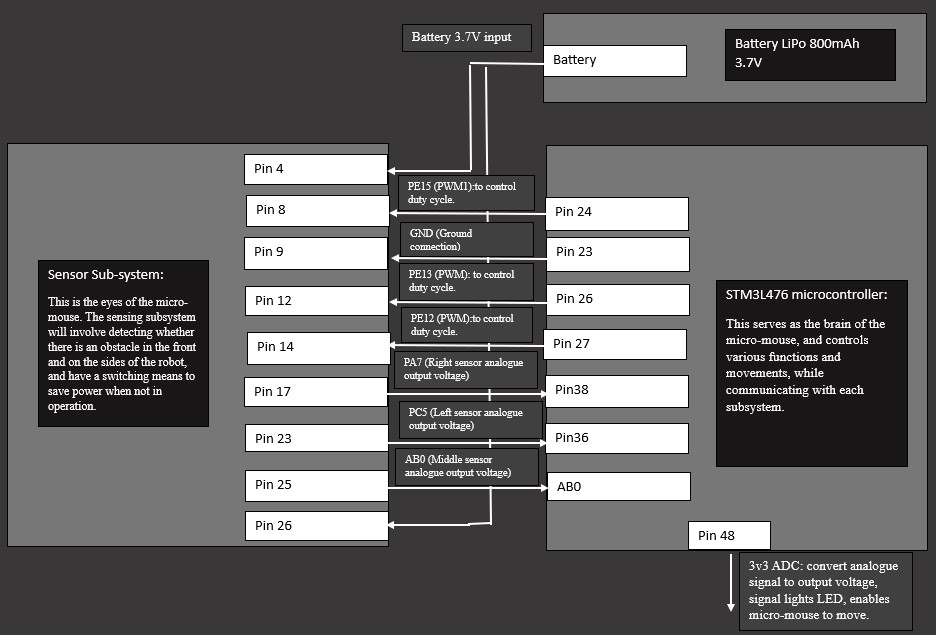
\includegraphics[width=1.1\linewidth]{EEE3088F_final_report_latex_template-2//Figures/Interfacing_Diagram.jpg}
    \caption{High level block diagram}
    \label{fig:interface_diagram} 
\end{figure} \FloatBarrier






% ----------------------------------------------------
\end{document}
% ----------------------------------------------------